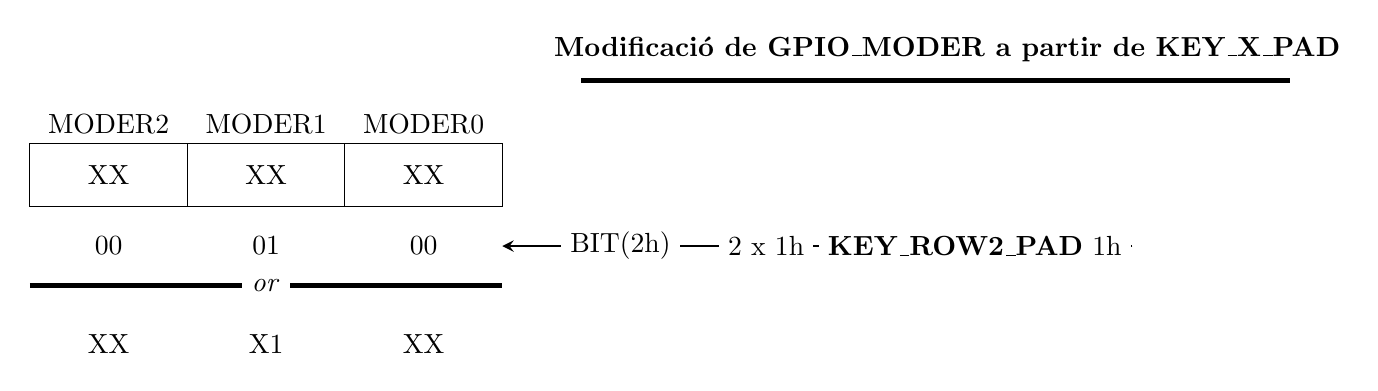
\begin{tikzpicture}
    \draw[ultra thick] (7, 1.6) -- (16, 1.6);
    \node[] at(11.65, 2) {\textbf{Modificació de GPIO\_MODER a partir de KEY\_X\_PAD}};

    \foreach \i in {0,...,2}
    {\node[above] at (5 -2*\i, 0.8) {MODER\i};}
    \foreach \i in {0,...,2}
    {\draw[] (2*\i, 0) rectangle ++(2, 0.8);}
    \foreach \i in {0,...,2}
    {\node[] at (1+2*\i, 0.4) {XX};}

    \draw[thick, -stealth] (14, -0.5) -- (6, -0.5);

    \node[] at(3, -0.5) {$01$};
    \node[] at(5, -0.5) {$00$};
    \node[] at(1, -0.5) {$00$};

    \node[fill=white] at(12, -0.5){\textbf{KEY\_ROW2\_PAD} 1h};
    \node[fill=white] at(9.35, -0.5){2 x 1h};
    \node[fill=white] at(7.5, -0.5){BIT(2h)};

    \draw[ultra thick] (0, -1) -- ++ (6, 0);
    \node[fill=white] at(3, -1){\textit{or}};

    \node[] at(3, -1.75) {X1};
    \node[] at(5, -1.75) {XX};
    \node[] at(1, -1.75) {XX};
\end{tikzpicture}